
\documentclass[12pt,onecolumn]{article}
\usepackage[brazilian]{babel}
\usepackage[utf8]{inputenc}
\usepackage{hyperref}
\usepackage[section]{placeins}
\usepackage{graphicx}
\usepackage{caption}
\usepackage{subcaption}
\usepackage{float}
\usepackage{framed,color}

\begin{document}

% Title page.
\begin{titlepage}

    % Title info.
    \title{
        \bf
        \LARGE Apostila de \\
        \Huge  GIMP
    }
    
    \author{Renan Teruo Carneiro \\ Wilson Kazuo Mizutani}
    
    % Print title.
    \maketitle
    
    % No numbering on this page.
    \thispagestyle{empty}
    
\end{titlepage}

% Print table of contents.
\tableofcontents

% Page break.
\clearpage

\section{Sobre o GIMP}
  Do site oficial do GIMP (\url{http://gimp.org}):
  
  \begin{quotation}
    GIMP is an acronym for GNU Image Manipulation Program. It is a freely
    distributed program for such tasks as photo retouching, image composition
    and image authoring.
  \end{quotation}
  
  Além disso, o GIMP possui atualmente uma vasta comunidade de usuários. Cada
  vez mais ele representa uma alternativa efetiva aos programas de manipulação
  de imagem comerciais. Seus usos variam desde {\it pixel art} até
  elaboradíssimas edições e composições de fotos e cenários.
  
  \vspace{50pt}
  
  \begin{figure}[ht]
    \centering
    \begin{subfigure}{.5\textwidth}
      \centering
      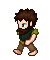
\includegraphics[width=.7\linewidth]{screenshots/00-pixel_art.png}
      \caption{
        \footnotesize
        \it
        Pixel Art
      }
    \end{subfigure}%
    \begin{subfigure}{.5\textwidth}
      \centering
      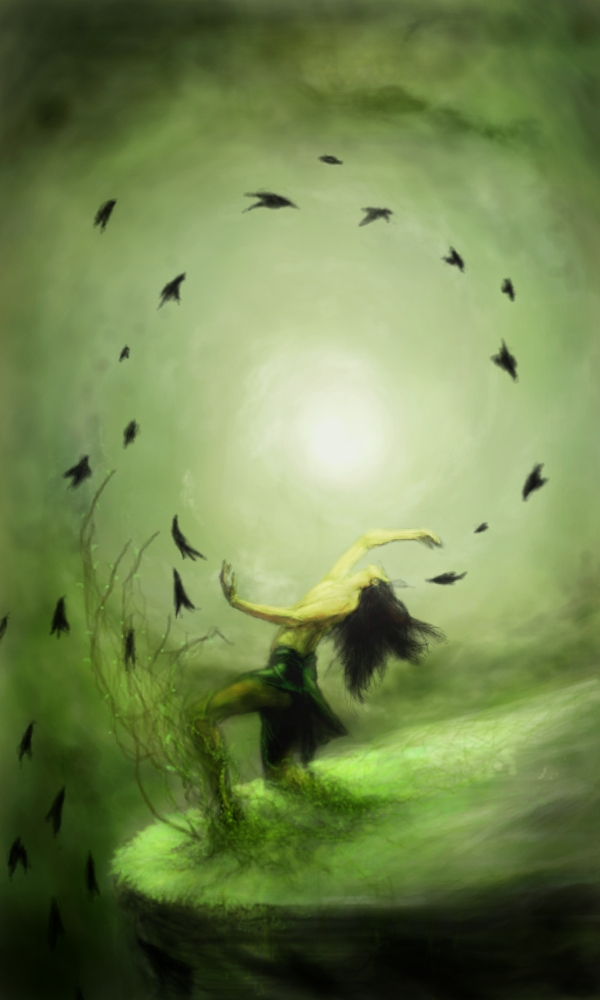
\includegraphics[width=.7\linewidth]{screenshots/Dance_of_Rebirth_by_shiroikuro.jpg}
      \caption{
        \footnotesize
        \it
        Concept Art
      }
    \end{subfigure}
    \caption{
      \footnotesize
      \it
      Imagens feitas no GIMP.
    }
  \end{figure}

\clearpage
\section{Instalando}
  O site oficial do GIMP oferece instruções diretas de como instalar o {\it
  software} na sua máquina de interesse:
  
  \begin{center}
    \url{http://www.gimp.org/downloads/}
  \end{center}
  
  O único detalhe é que estamos usando a versão 2.8 (principalmente devido à
  funcionalidade {\it Single-Window Mode}). Se você usa Windows, então é só
  usar o link do site para baixar o instalador. Mas, se você usa Linux, talvez
  seja preciso adicionar algum repositório na lista do seu gerenciador de 
  pacotes caso ele esteja desatualizado. De qualquer maneira, o site explica
  como lidar com esse tipo de situação.

\clearpage
\section{Introdução}
  Como uma introdução ao GIMP, vamos fazer uma edição bem simples. O objetivo
  será colorir a imagem de um ícone preto-e-branco, como mostrado na Figura
  \ref{fig:intro}. A imagem original está disponível em
  
  \begin{center}
    \url{http://game-icons.net/lorc/original/beast-eye.html}      
  \end{center}
  
   O ideal é pegar a versão com maior resolução possível, em PNG.

  \begin{figure}
  \centering
  \begin{subfigure}{.5\textwidth}
    \centering
    
\includegraphics[width=.7\linewidth]{beast-eye.png}
    \label{fig:ex1_before}
  \end{subfigure}%
  \begin{subfigure}{.5\textwidth}
    \centering
    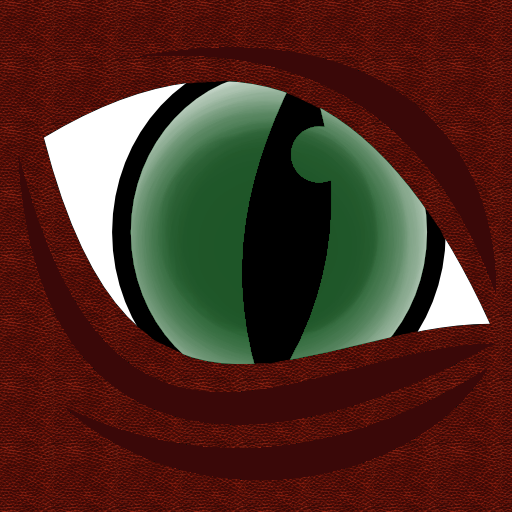
\includegraphics[width=.7\linewidth]{draft00.png}
    \label{fig:ex1_after}
  \end{subfigure}
  \caption{
    \footnotesize
    \it
    Imagem antes e depois da edição
  }
  \label{fig:intro}
  \end{figure}
  
  Com esse exercício esperamos apresentar as funcionalidades básicas e as
  técnicas essenciais para se manipular imagens com o GIMP. Mas apesar do foco
  nesse momento ser passar os conceitos básicos para o aluno, também
  introduziremos algumas das principais ferramentas usadas em projetos GIMP.
  
  \subsection{Abrindo a imagem e convertendo para RGBA}
    O primeiro passo do exercício é dizer para o GIMP que queremos trabalhar em
    RGBA (isso é, com cores e transparência) ao invés de Grayscale, que é o
    formato no qual a imagem do ícone está. E vamos aproveitar esse passo para
    mostrar o básico de copiar e colar imagens com GIMP (que não é muito
    diferente do convencional).
    
    Começamos abrindo a imagem original indo em {\bf File $\rightarrow$ Open}
    ou digitando {\bf CTRL+O}.
    
    \begin{framed}
      Algo que facilita muito o uso do GIMP é a familiarização com os atalhos
      de teclado. Saber uma meia-dúzia de atalhos é o suficiente para dobrar a
      eficiência de trabalho. 
    \end{framed}
    
    Do jeito que o GIMP carrega a imagem (em Grayscale) não é possível aplicar
    nenhuma cor aos pixeis. Isso significa que se selecionarmos, por exemplo,
    a {\bf Pencil Tool} (atalho {\bf N}), e mudarmos a cor para vermelho, ainda
    assim pintaremos apenas tons de cinza.
    
    \begin{framed}
      Para mudar de cor no GIMP, basta clicar duas vezes no retângulo colorido
      no meio da {\bf Toolbox }, como mostra a Figura \ref{fig:pencil_and_color}.
    \end{framed}
    
    \begin{figure}[ht]
      \centering
      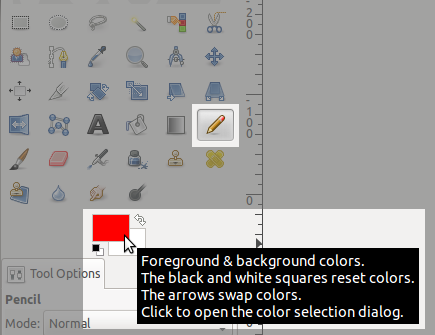
\includegraphics[width=.6\textwidth]{screenshots/00-pencil_and_color.png}
      \caption{
        \footnotesize
        \it
        Seleciondo a {\bf Pencil Tool} e mudando a cor.
      }
      \label{fig:pencil_and_color}
    \end{figure}
    
    \begin{framed}
      Para desfazer uma ação GIMP, pode-se ir em {\bf Edit $\rightarrow$ Undo}
      ou digitar {\bf CTRL+Z}. É um comando {\it extremamente útil}, e o
      histórico de ações que o GIMP guarda é bastante grande. Use ele para
      desfazer quaisquer alterações que você possa ter feito na imagem original
      antes de seguir os próximos passos.
    \end{framed}
    
    Vamos, então, criar uma nova imagem que use RGBA ao invés de Grayscale. Para
    isso, clicamos em {\bf File $\rightarrow$ New} ou digitamos {\bf CTRL+N}. Um
    menu {\bf Create a New Image} aparecerá. Nele temos acesso à várias
    configurações da nova imagem, como a largura e a altura dela. Essas
    manteremos como estão (512x512 se você pegou a maior resolução disponível).
    O que nos interessa aqui é mudar o formato de cores e o suporte a
    transparência. Basta mudar essas configurações conforme a Figura
    \ref{fig:grayscale_to_RGBA}.
    
    \begin{figure}[H]
      \centering
      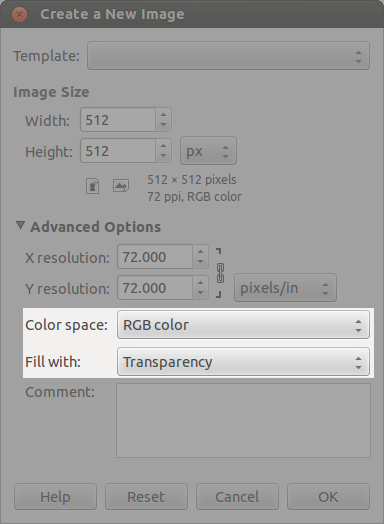
\includegraphics[scale=.55]{screenshots/00-grayscale_to_RGBA.png}
      \caption{
        \footnotesize
        \it
        Criando uma imagem RGBA
      }
      \label{fig:grayscale_to_RGBA}
    \end{figure}
    
    Uma vez feito isso, basta voltarmos para a imagem original, e:
    
    \begin{itemize}
      \item
        Selecionarmos ela inteira com {\bf Botão Direito do Mouse $\rightarrow$
        Selection $\rightarrow$ All} ou {\bf CTRL+A}.
      \item
        Copiarmos ela com {\bf Botão Direito do Mouse $\rightarrow$ Edit
        $\rightarrow$ Copy} ou {\bf CTRL+C}.
      \item
        Voltarmos para a imagem com RGBA que acabamos de criar.
      \item
        Colarmos o ícone orignal nela com {\bf Botão Direito do Mouse
        $\rightarrow$ Edit $\rightarrow$ Paste} ou {\bf CTRL+V}.
    \end{itemize}
    
    
  \subsection{Sobre seleções}
    Agora que temos nossa imagem pronta para ser manipulada, vamos falar sobre
    seleções no GIMP. Seleções são um conceito primordial para qualquer tipo de
    edição, pois {\bf toda ferramenta que não seja de seleção, só é aplicada
    sobre a seleção atual}. Quando não há nenhuma seleção, então a imagem toda
    é considerada selecionada (ou seja, as ferramentas serão aplicadas em todas
    as partes dela).
    
    Para entender isso melhor, podemos escollher a {\bf Rectangle Selection
    Tool} (atalho {\bf R}) e selecionar uma região qualquer da imagem
    clicando e arrastando o mouse, e depois soltando-o. Agora, se escolhermos,
    por exemplo, a {\bf Bucket Feel Tool} (atalho {\bf SHIFT+B}) e tentarmos
    usá-la, obteremos o resultado mostrado na Figura
    \ref{fig:selective_painting}.
  
    \begin{figure}[H]
      \centering
      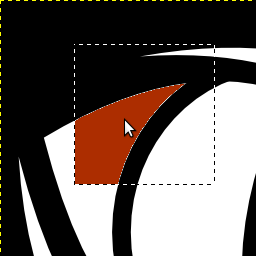
\includegraphics[scale=0.6]{screenshots/01-selective_painting.png}
      \caption{
        \footnotesize
        \it
        As ferramentas trabalham apenas nas regiões selecionadas
      }
      \label{fig:selective_painting}
    \end{figure}
    
    Outras duas ferramentas de seleção que vamos usar bastante são a {\bf
    Free Select Tool} (atalho {\bf F}) e a {\bf Fuzzy Select Tool} (atalho
    {\bf U}). A primeira permite selecionar uma região à mão livre e a segunda
    seleciona uma região que tenha uma cor em comum. Recomendamos experimentar
    um pouco com ela antes de prosseguir. Possíveis resultados do uso dessas
    ferramentas podem ser vistas na Figura \ref{fig:select_tools}.
    
    \begin{framed}
      A {\bf Free Select Tool} também pode ser usada traçando retas. Cada ponto
      que você clicar será ligado ao anterior, até que você volte a clicar no
      primeiro. Então, a região será selecionada. Também é possível misturar
      trechos retos e à mão livre.
    \end{framed}
    
    \begin{figure}[ht]
      \centering
      \begin{subfigure}{.5\textwidth}
        \centering
        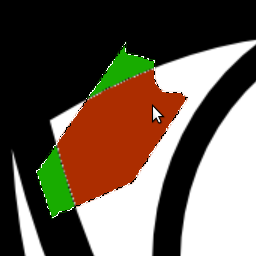
\includegraphics[width=.7\linewidth]{screenshots/02-free_select.png}
        \label{fig:free_select}
      \end{subfigure}%
      \begin{subfigure}{.5\textwidth}
        \centering
        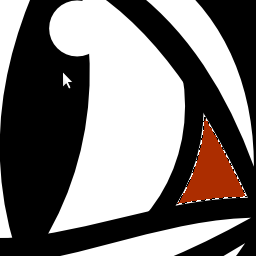
\includegraphics[width=.7\linewidth]{screenshots/03-fuzzy_select.png}
        \label{fig:fuzzy_select}
      \end{subfigure}
      \caption{
        \footnotesize
        \it
        Free Select Tool (esquerda) e Fuzzy Select Tool (direita).
      }
      \label{fig:select_tools}
    \end{figure}
  
    Agora, vamos afazer algo mais útil. Vamos colorir a pupila do olho na
    imagem. Como é de se esperar, para isso precisamos selecionar a pupila. A
    primeira ideia é usar a {\bf Fuzzy Selection Tool} e clicar nas regiões que
    correspondem à pupila. No entanto, como nas bordas dessa região há uma
    transição do branco para o preto, a seleção não fica perfeita (partes da
    borda ficam de fora). Além disso, mesmo que selecionássemos um dos lados da
    pupila, como selecionar o outro ao mesmo tempo?
    
    \begin{figure}[ht]
      \centering
      
\includegraphics[width=.5\textwidth]{screenshots/04-pupil.png}
      \caption{
        \footnotesize
        \it
        O objetivo é selecionar apenas a pupila para podermos manipulá-la sem
        correr o risco de "vazar" para as outras partes da imagem
      }
      \label{fig:pupil}
    \end{figure}
    
    É nesse ponto que entram as {\bf operações de seleção}. Começando pelo
    primeiro problema, o grande obstáculo é que a {\bf Fuzzy Selection Tool} não
    alcança todas as partes da região branca, isso é, fica {\it faltando pixels}
    na região selecionada e {\it sobrando} na região não selecionada. Por outro
    lado, o mesmo acontece se a usamos para selecionar a região preta. Então uma
    plausível solução seria pegarmos o {\it inverso} da região preta. A {\bf
    operação de inversão} é a primeira das operações de seleção, e pode ser
    realizada usando {\bf Botão Direito do Mouse $\rightarrow$ Select
    $\rightarrow$ Invert} ou {\bf CTRL+I}.
    
    Mas então temos outro problema: todas as regiões brancas ficaram
    selecionadas. Para resolver isso usamos a {\bf operação de intersecção} ou
    a {\bf operação de diferença}. Diferentemente da operação de inversão, essas
    operações são aplicadas com o auxílio de alguma ferramenta de seleção. No
    caso, vamos usar a {\bf Free Select Tool}.
    
    Para ativar a operação de intersecçao, basta segurar {\bf CTRL+SHIFT} e usar
    a ferramenta de seleção. Quando terminar, {\bf todas as regiões em comum}
    entre a região até então selecionada e a nova comporão a nova seleção.
    
    Para ativar a operação de diferença, deve-se segurar {\bf CTRL} e usar a
    ferramenta de seleção. No final, as novas regiões selecionadas serão {\bf
    subtraídas} da seleção antiga.
    
    \begin{framed}
      A última operação de seleção é a {\bf operação de soma}. Ela é ativada
      segurando {\bf SHIFT} antes de usar uma ferramenta de seleção, e a nova
      região selecionada é somada à que havia antes.
    \end{framed}
    
    \begin{figure}[ht]
      \centering
      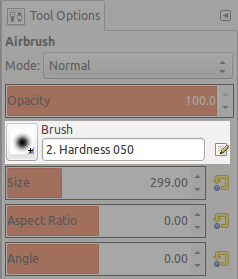
\includegraphics[width=.5\textwidth]{screenshots/04-setting_brush.png}
      \caption{
        \footnotesize
        \it
        Muda-se o pincel ({\it brush}) usado por uma ferramenta de manipulação
        na região destacada.
      }
      \label{fig:setting_brush}
    \end{figure}
    
    Quando, enfim, a pupila estiver devidamente selecionada, use alguma
    ferramenta de manipulação para deixá-la como preferir. No nosso exemplo,
    usamos a {\bf Airbrush Tool}. Ajustamos o formato do pincel dela na opção
    indicada na Figura \ref{fig:setting_brush}, e aumentamos seu tamanho até
    ficar do tamanho da pupila. Por fim, aplicamos ela no centro da pupila (que,
    em particular, não está na região selecionada) e obtivemos o resultado da
    Figura \ref{fig:pupil}.
    
    \begin{framed}
      Para diminuir ou aumentar o tamanho de uma ferramenta de manipulação,
      usa-se os botões {\bf \verb$[$} e {\bf \verb$]$}, respectivamente.
    \end{framed}
        
  \subsection{Sobre camadas}
    
    Uma dificuldade comum quando se começa a usar o GIMP é saber como mover
    seleções. Quando tentamos mover uma região selecionada usando a {\bf Move
    Tool}, por exemplo, apenas o contorno da região se move, e não o conteúdo
    dela. Para fazer isso, é preciso recortar e logo em seguida colar de volta a
    região selecionada. Só então é que a região junto com seu conteúdo poderá
    ser movida.
    
    \begin{framed}
      Para recortar podemos usar {\bf Botão Direito do Mouse $\rightarrow$ Edit
      $\rightarrow$ Cut} ou o atalho {\bf CTRL+X}.
    \end{framed}
    
    Na verdade, o que acontece é que quando colamos algo no GIMP, uma nova {\it
    camada} é criada usando a seleção colada. E, assim, quando movemos a
    seleção, estamos realmente é movendo a nova camada. Quando confirmamos a
    colagem (clicando fora da seleção, normalmente), essa camada temporária
    criada pelo GIMP é aplicada na original. Ela recebe o nome de {\it Floating
    Selection} enquanto estiver nesse estado intermediário, como mostra a figura
    \ref{fig:pasted_layer}.
    
    Mas qual a utilidade das camadas? Assim como com as seleções, {\bf as
    ferramentas de edição do GIMP são aplicadas apenas na camada atualmente
    selecionada}. Ou seja, no final das contas {\bf as ferramentas de edição só
    funcionam na seleção atual da camada focada}. Mas as camadas, diferentemente
    de simples seleções, têm a vantagem de persistirem ao longo do projeto. Você
    pode dividir seu trabalho em camadas, e trabalhar separadamente em cada uma
    sem que haja interferência entre elas. Sempre que quiser voltar a mexer em
    uma delas basta selecioná-la no menu {\bf Layers}.
    
    \begin{figure}[H]
      \centering
      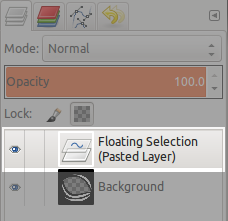
\includegraphics[width=.5\textwidth]{screenshots/05-pasted_layer.png}
      \caption{
        \footnotesize
        \it
        Seleções coladas ficam em uma camada flutuante temporária
      }
      \label{fig:pasted_layer}
    \end{figure}
    
    Então, voltando ao nosso exercício, vamos selecionar o olho inteiro e
    separá-lo em uma camada diferente do resto. Para isso, vamos nos aproveitar
    do mecanismo de recortar e colar que acabamos de ver. Usando as ferramentas
    de seleção {\bf Free} e {\bf Fuzzy}, junto com as operações de seleção,
    selecionamos o olho e o recortamos, para depois colar de volta. Só que ao
    invés de simplesmente confirmamos a colagem, vamos usar {\bf Botão Direito
    do Mouse $\rightarrow$ To New Layer} sobre a camada flutuante no menu de
    camadas. Isso irá de fato isolar a seleção em uma nova camada, como
    queremos.
    
    Mas a nova camada criada estará com um nome parecido com {\it Pasted Layer}
    ou algo assim. Para mudar isso, basta selecioná-la no menu de camadas e usar
    {\bf Botão Direito do Mouse $\rightarrow$ Edit Layer Attributes} ou apertar
    o botão {\bf F2}. Podemos renomear a camada do olho para "Eye", por exemplo.
    Eventualmente, se quisermos remover uma camada, é só clicar nela e usar
    {\bf Botão Direito do Mouse $\rightarrow$ Delete Layer} (note que pressionar
    {\bf DELETE} terá um efeito completamente diferente: ele irá apagar todo o
    conteúdo da camada, deixando apenas pixeis transparentes ou da cor de fundo,
    dependendo do tipo da imagem).
    
    Além disso, como é possível perceber, o GIMP apresenta as camadas de baixo
    para cima, isso é, as camadas de cima aparecem por cima das camadas de
    baixo. É possível alterar essa ordem clicando e arrastando elas no menu de
    camadas. Também é possível ocultar uma camada clicando no ícone de olho do
    lado esquerdo do nome delas (vide Figura \ref{fig:hide_layer}).
    
    \begin{figure}[H]
      \centering
      
\includegraphics[width=.5\textwidth]{screenshots/06-hide_layer.png}
      \caption{
        \footnotesize
        \it Podemos esconder uma camada clicando no ícone destacado
      }
      \label{fig:hide_layer}
    \end{figure}
    
    \begin{framed}
      É importante ressaltar que quando exportamos um trabalho para, digamos,
      uma imagem PNG, a imagem final será uma sobreposição apenas das camadas
      visíveis (as ocultas não aparecerão).
    \end{framed}
    
    Outro detalhe de criar camadas recortando e colando é que a nova camada
    acaba tendo {\it um tamanho menor que a orignal}. Esse tamanho pode ser
    reconhecido por uma linha pontilhada preta e amarela em volta da região que
    delimita a camada. Para ajustar ela de volta para o tamanho total da imagem,
    usa-se {\bf Botão Direito do Mouse $\rightarrow$ Layer to Image Size}.
    
    
    Mas agora a camada de baixo (provavelmente chamada de {\it beast-eye.png})
    ficou com um espaço vazio onde o olho ficava. Podemos facilmente preencher
    ele de preto usando a {\bf Bucket Fill Tool} mencionada mais cedo. Vamos
    aproveitar para renomear essa camada para "Background" ou algo semelhante
    que faça sentido. Depois, vamos repetir o processo de criar uma nova camada
    para as estrias do desenho, e chamemos essa terceira camada de algo como
    "Stripes". No final, o esquema de camadas deve estar condizente com a Figura
    \ref{fig:layers}.
    
    \begin{figure}[ht]
      \centering
      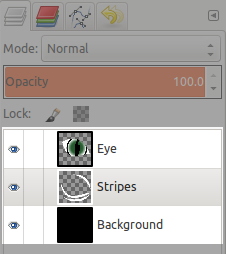
\includegraphics[width=.5\textwidth]{screenshots/07-layers.png}
      \caption{
        \footnotesize
        \it
        As três camadas no final
      }
      \label{fig:layers}
    \end{figure}
    
  \subsection{Finalizando}
  
    Bom, agora que a imagem está devidamente separada em camadas, falta apenas
    colorí-las apropriadamente. Podemos pintar as estrias com uma única cor
    usando a técnica de inverter a seleção do fundo pela Fuzzy Selection Tool e
    depois aplicar a Bucket Fill Tool sobre as regiões selecionadas resultantes.
    Poderíamos usar qualquer outra ferramenta de edição além da Bucket, mas por
    simplicidade vamos continuar usando ela de exemplo. Nesse ponto, teremos
    algo parecido com o que aparece na Figura \ref{fig:partial}.
    
    \begin{figure}[ht]
      \centering
      
\includegraphics[width=.3\textwidth]{screenshots/06-partial.png}
      \caption{
        \footnotesize
        \it
        Resultado quase pronto da edição
      }
      \label{fig:partial}
    \end{figure}
    
    Vamos, por fim, colorir o fundo. Nesse caso, como queremos preencher toda a
    camada em questão, não precisamos nos preocupar com seleções. Mais uma vez
    usaremos a ferramente Bucket, mas agora com uma textura ao invés de uma
    simples cor plana. Para tanto, selecionamos a opção {\bf Pattern Fill} no
    menu da ferramenta Bucket (metade de baixo do menu Toolbox) e mudamos a
    textura desejada para {\it Leather}, por exemplo. Esse passos estão expostos
    na Figura \ref{fig:pattern_fill}.
    
    \begin{figure}[ht]
      \centering
      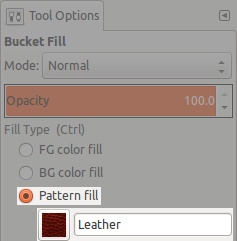
\includegraphics[width=.4\linewidth]{screenshots/07-pattern_fill.png}
      \caption{
        \footnotesize
        \it
        Ajustando a ferramenta Bucket para usar a textura Leather
      }
      \label{fig:pattern_fill}
    \end{figure}
    
    Agora é só aplicar a ferramenta Bucket na camada de fundo! Com isso chegamos
    ao resultado final mostrado no começo da introdução, mostrado na Figura
    \ref{fig:final}. Mas um dos problemas da imagem do jeito que ela ficou é que
    ela está muito {\it plana}. É possível usar diversas ferramentas de edição
    para melhorar isso. O leitor pode consultar a seção de ferramentas em
    busca da que achar melhor, mas sugerimos a {\bf Dodge/Burn Tool} para
    efeitos de luz e sombra, por exemplo. Também vale a pena uma olhada na seção
    \ref{sec:color_control} ({\bf Controle de Cor}).
    
    \begin{figure}
      \centering
      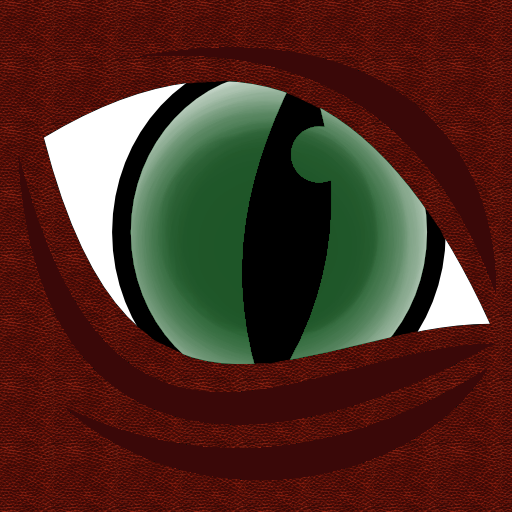
\includegraphics[width=\linewidth]{draft00.png}
      \caption{
        \footnotesize
        \it
        Resultado final
      }
      \label{fig:final}
    \end{figure}
    
    Também serve como um treino interessante repetir esse exercício usando
    ferramentas de edição diferentes e usando a própria criatividade. Por
    exemplo, poder-se-ia fazer uma pupila com efeitos mais interessantes.
    Muitas outras imagens semelhantes à usada podem ser encontradas e usadas
    gratuitamente do site:
    
    \begin{center}
      \url{http://game-icons.net/}
    \end{center}
      
    Contanto que seja dado o devido crédito ao autor.
    
\clearpage
\section{Ferramentas}

  \subsection{Seleção}
    \subsubsection{Retângulo}
      \begin{figure}[H]
        Atalho {\bf R}, Ícone 
        
\includegraphics{gimp-icons/stock-tool-rect-select-22.png}
        \label{fig:rectselect}
      \end{figure}
      Essa ferramenta seleciona uma área retângular. Para usá-la, basta selecionar um ponto,
      clicar e arrastar.

      \subsubsection{Elipse}
      \begin{figure}[H]
        Atalho {\bf E}, Ícone 
        
\includegraphics{gimp-icons/stock-tool-ellipse-select-22.png}
        \label{fig:ellipseselect}
      \end{figure}
      Essa ferramenta seleciona uma área elíptica. Para usá-la, basta selecionar um ponto,
      clicar e arrastar.

      \subsubsection{Livre}
      \begin{figure}[H]
        Atalho {\bf F}, Ícone
        
\includegraphics{gimp-icons/stock-tool-free-select-22.png}
        \label{fig:freeselect}
      \end{figure}
      Essa ferramenta seleciona uma área definida pelo usuário, sem ajustes. Para usá-la, basta
      selecionar um ponto, clicar e arrastar.
      
      \subsubsection{Tesoura}
      \begin{figure}[H]
        Atalho {\bf I}, Ícone
        
\includegraphics{gimp-icons/stock-tool-iscissors-22.png}
        \label{fig:scissorsselect}
      \end{figure}
      Essa ferramenta seleciona uma área definida pelo usuário, mas tentando separar áreas pela
      diferença de cores. Para usá-la, clique num ponto inicial, e em seguida clique nos pŕoximos
      pontos que contornam a área que você quer selecionar. Caso você queira mudar a seleção feita
      pelo GIMP, você pode clicar na borda da área selecionada e arrastar para onde ela deveria 
      estar.

      \subsubsection{Fuzzy}
      \begin{figure}[H]
        Atalho {\bf U}, Ícone
        
\includegraphics{gimp-icons/stock-tool-fuzzy-select-22.png}
        \label{fig:magicselect}
      \end{figure}
      Essa ferramenta seleciona uma área de cores semelhantes a uma área clicada inicialmente.
      A sensitividade da seleção pode ser alterada mantendo o botão do mouse pressionado e movendo
      o mouse.

      \subsubsection{Cor}
      \begin{figure}[H]
        Atalho {\bf Shift + O}, Ícone
        
\includegraphics{gimp-icons/stock-tool-by-color-select-22.png}
        \label{fig:colorselect}
      \end{figure}
      Essa ferramenta é parecida com a ferramente de seleção fuzzy, mas ela seleciona todas as áreas
      com cores semelhantes à área clicada. A sensitividade da seleção pode ser alterada do mesmo
      modo.

            
      

  \subsection{Edição}
    \subsubsection{Blur}
      \begin{figure}[H]
        Atalho {\bf Shift + U}, Ícone
        
\includegraphics{gimp-icons/stock-tool-blur-22.png}
        \label{fig:blur}
      \end{figure}
      O blur suaviza a área afetada, dando uma impressão de embaçamento.
      %%TODO: Exemplificar através de imagem

  \subsubsection{Bucket Fill}
      \begin{figure}[H]
        Atalho {\bf Shift + B}, Ícone
        
\includegraphics{gimp-icons/stock-tool-bucket-fill-22.png}
        \label{fig:bucket}
      \end{figure}
      O bucket fill preenche toda uma área de uma determinada cor com outra cor.
    
    \subsubsection{Clone}
      \begin{figure}[H]
        Atalho {\bf C}, Ícone
        
\includegraphics{gimp-icons/stock-tool-clone-22.png}
        \label{fig:clone}
      \end{figure}
      A ferramenta clone copia uma área origem da imagem em outra área destino da imagem.
      
    \subsubsection{Heal}
      \begin{figure}[H]
        Atalho {\bf H}, Ícone
        
\includegraphics{gimp-icons/stock-tool-heal-22.png}
        \label{fig:heal}
      \end{figure}
      A ferramente heal é parecida com a clone, mas a imagem é copiada de maneira mais suave.

    \subsubsection{Color Picker}
      \begin{figure}[H]
        Atalho {\bf O}, Ícone
        
\includegraphics{gimp-icons/stock-tool-color-picker-22.png}
        \label{fig:color-picker}
      \end{figure}
      Essa ferramenta seleciona a cor do pixel clicado.
      
    \subsubsection{Dodge}
      \begin{figure}[H]
        Atalho {\bf Shift + D}, Ícone
        
\includegraphics{gimp-icons/stock-tool-dodge-22.png}
        \label{fig:dodge}
      \end{figure}
      Essa ferramenta clareia ou escurece a área afetada. Para escurecer, segure shift ao clicar.

    \subsubsection{Eraser}
      \begin{figure}[H]
        Atalho {\bf Shift + E}, Ícone
        
\includegraphics{gimp-icons/stock-tool-eraser-22.png}
        \label{fig:eraser}
      \end{figure}
      Essa ferramenta apaga a área afetada. Se a camada possui um canal alpha, a parte apagada ficará
      transparente. Caso contrário, ficará da cor secundária.


    \subsubsection{Move}
      \begin{figure}[H]
        Atalho {\bf M}, Ícone
        
\includegraphics{gimp-icons/stock-tool-move-22.png}
        \label{fig:move}
      \end{figure}
      Move a imagem, camada atual ou área de seleção. Note que, se estiver no modo de mover área de
      seleção, ele move a área de seleção em si, não a área selecionada.

    \subsubsection{Paintbrush}
      \begin{figure}[H]
        Atalho {\bf P}, Ícone
        
\includegraphics{gimp-icons/stock-tool-paintbrush-22.png}
        \label{fig:brush}
      \end{figure}
      Pinta suavemente da cor escolhida. O estilo do pincel pode ser escolhido.
      
    \subsubsection{Pencil}
      \begin{figure}[H]
        Atalho {\bf N}, Ícone
        
\includegraphics{gimp-icons/stock-tool-pencil-22.png}
        \label{fig:pencil}
      \end{figure}
      Pinta toda a área do pincel, sem suavizações.
      
    \subsubsection{Rotate}
      \begin{figure}[H]
        Atalho {\bf Shift + R}, Ícone
        
\includegraphics{gimp-icons/stock-tool-rotate-22.png}
        \label{fig:rotate}
      \end{figure}
      Rotaciona a área selecionada.
      
    \subsubsection{Scale}
      \begin{figure}[H]
        Atalho {\bf Shift + T}, Ícone
        
\includegraphics{gimp-icons/stock-tool-scale-22.png}
        \label{fig:scale}
      \end{figure}
      Altera o tamanho da área selecionada.

    \subsubsection{Smudge}
      \begin{figure}[H]
        Atalho {\bf S}, Ícone
        
\includegraphics{gimp-icons/stock-tool-smudge-22.png}
        \label{fig:smudge}
      \end{figure}
      Borra a área afetada, de maneira semelhante a alguém passando o dedo por cima.
      
    \subsubsection{Text}
      \begin{figure}[H]
        Atalho {\bf T}, Ícone
        
\includegraphics{gimp-icons/stock-tool-text-22.png}
        \label{fig:text}
      \end{figure}
      Insere um texto na imagem.

  \subsection{Controle de Cor}
  \label{sec:color_control}
  
    Muitas vezes queremos apenas mudar as cores de uma imagem, e ter que editar
    manualmente seria exaustivo senão inviável. Por exemplo, se quisermos passar
    parte de uma imagem colorida para tons de cinza, podemos usar tanto a opção
    {\bf Hue-Saturation} como a {\bf Colorize} para retirar toda a saturação da
    imagem.
    
    \begin{framed}
      Além do formato usual de representação de cores RGB, também é possível
      existe o Hue-Saturaion-Lightness, que em geral é mais fácil e mais
      intuitivo de usar. Como o próprio nome indica, você escolhe valores de
      matiz, saturação e luminosidade da cor.
    \end{framed}
    
    Essas opções podem ser encontradas no menu {\bf Colors}. Nessa apostila,
    explicamos apenas as quatro primeiras, que são as mais simples e mais úteis
    de maneira geral.
    
    Assim como as ferramentas, essas opções são aplicadas sobre a seleção atual,
    ou sobre a camada inteira se não houver seleção.
    
      \subsubsection{Color Balance}
        Essa opção permite que você manipule a proporção das cores, alterando o
        balanço entre as partes complementares. Você pode, por exemplo, aumentar
        a proporção de amarelo diminuindo a parte azul, e toda a região afetada
        ficará mais amarelada.
      
        \begin{figure}[H]
          \centering
          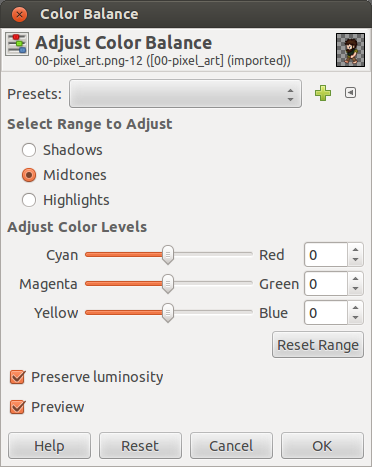
\includegraphics[width=.6\linewidth]{screenshots/08-color_balance.png}
          \caption{
            \footnotesize
            \it
            Menu de controle de balanço de cores.
          }
          \label{fig:color_balance}
        \end{figure}
        
        No entanto, a opção atinge apenas certos intervalos de cores. Como pode
        ser visto na Figura \ref{fig:color_balance}, você pode escolher qual
        intervalo afetar dentre sombras, tons médios e iluminações.
        
        Essa opção pode ser usada para ajustar os tons das cores de imagens. Por
        exemplo, é possível manipular a iluminação em uma foto de forma a fazer
        parecer que a luz no local é de uma cor diferente da original.
      
      \subsubsection{Hue-Saturation}
      
      \subsubsection{Colorize}
      
      \subsubsection{Brightness-Contrast}

\end{document}
